%%% Hlavní soubor. Zde se definují základní parametry a odkazuje se na ostatní části. %%%

%% Verze pro jednostranný tisk:
% Okraje: levý 40mm, pravý 25mm, horní a dolní 25mm
% (ale pozor, LaTeX si sám přidává 1in)
\documentclass[12pt,a4paper]{report}
\setlength\textwidth{145mm}
\setlength\textheight{247mm}
\setlength\oddsidemargin{15mm}
\setlength\evensidemargin{15mm}
\setlength\topmargin{0mm}
\setlength\headsep{0mm}
\setlength\headheight{0mm}
% \openright zařídí, aby následující text začínal na pravé straně knihy
\let\openright=\clearpage

%% Pokud tiskneme oboustranně:
% \documentclass[12pt,a4paper,twoside,openright]{report}
% \setlength\textwidth{145mm}
% \setlength\textheight{247mm}
% \setlength\oddsidemargin{14.2mm}
% \setlength\evensidemargin{0mm}
% \setlength\topmargin{0mm}
% \setlength\headsep{0mm}
% \setlength\headheight{0mm}
% \let\openright=\cleardoublepage

%% Vytváříme PDF/A-2u
\usepackage[a-2u]{pdfx}

%% Přepneme na českou sazbu a fonty Latin Modern
\usepackage[czech]{babel}
\usepackage{lmodern}
\usepackage[T1]{fontenc}
\usepackage{textcomp}

%% Použité kódování znaků: obvykle latin2, cp1250 nebo utf8:
\usepackage[utf8]{inputenc}

%%% Další užitečné balíčky (jsou součástí běžných distribucí LaTeXu)
\usepackage{amsmath}        % rozšíření pro sazbu matematiky
\usepackage{amsfonts}       % matematické fonty
\usepackage{amsthm}         % sazba vět, definic apod.
\usepackage{bbding}         % balíček s nejrůznějšími symboly
			    % (čtverečky, hvězdičky, tužtičky, nůžtičky, ...)
\usepackage{bm}             % tučné symboly (příkaz \bm)
\usepackage{graphicx}       % vkládání obrázků
\usepackage{fancyvrb}       % vylepšené prostředí pro strojové písmo
\usepackage{indentfirst}    % zavede odsazení 1. odstavce kapitoly
\usepackage{natbib}         % zajištuje možnost odkazovat na literaturu
			    % stylem AUTOR (ROK), resp. AUTOR [ČÍSLO]
\usepackage[nottoc]{tocbibind} % zajistí přidání seznamu literatury,
                            % obrázků a tabulek do obsahu
\usepackage{icomma}         % inteligetní čárka v matematickém módu
\usepackage{dcolumn}        % lepší zarovnání sloupců v tabulkách
\usepackage{booktabs}       % lepší vodorovné linky v tabulkách
\usepackage{paralist}       % lepší enumerate a itemize
\usepackage[usenames]{xcolor}  % barevná sazba

\usepackage{subcaption}
\usepackage{wrapfig}
%\usepackage{imakeidx}
\usepackage{makeidx}
\makeindex
%\makeindex[program=texindy,options=-L czech -M lang/czech/utf8 -M indexstyle.xdy]

\usepackage{filecontents}
\begin{filecontents*}{instyle.xdy}
;;; xindy style file

;;; Load a predefined style:
;;;(require "makeindex.xdy")


(markup-locclass-list :open ", " :sep "")

(define-attributes (( "textbf" "default" )) )
(markup-locref   :attr  "textbf"     :open "\textbf{\hyperpage{" :close "}}")
(markup-locref   :attr  "textit"     :open "\textit{\hyperpage{" :close "}}")
(markup-locref   :attr  "textttt"     :open "\textttt{\hyperpage{" :close "}}")
(markup-locref   :attr  "texttsc"     :open "\texttsc{\hyperpage{" :close "}}")
(markup-locref   :attr  "default"     :open "\hyperpage{" :close "}")



\end{filecontents*}


%%% Údaje o práci

\def\problemy{{\noindent\bf Problémy}\par\bigskip}
\def\TODO#1{{\bf\color{red}#1}\expandafter\expandafter\expandafter\def\expandafter\expandafter\expandafter\problemy\expandafter\expandafter\expandafter{\expandafter\problemy\thepage: #1\par}}

% Název práce v jazyce práce (přesně podle zadání)
\def\NazevPrace{Percepční učení a Ideální Bayesovský\jednoumezera pozorovatel při zrakovém vyhledávání}
\def\jednoumezera{\linebreak\par\vglue -14pt\noindent\global\def\jednoumezera{\ }}
% Název práce v angličtině
\def\NazevPraceEN{Perceptual learning and Ideal Bayesian observer in visual search task}

% Jméno autora
\def\AutorPrace{Viktor Němeček}

% Rok odevzdání
\def\RokOdevzdani{2018}

% Název katedry nebo ústavu, kde byla práce oficiálně zadána
% (dle Organizační struktury MFF UK, případně plný název pracoviště mimo MFF)
\def\Katedra{Katedra softwaru a výuky informatiky}
\def\KatedraEN{Department of Software and Computer Science Education}

% Jedná se o katedru (department) nebo o ústav (institute)?
\def\TypPracoviste{Katedra}
\def\TypPracovisteEN{Department}

% Vedoucí práce: Jméno a příjmení s~tituly
\def\Vedouci{Mgr. Filip Děchtěrenko, Ph.D.}

% Pracoviště vedoucího (opět dle Organizační struktury MFF)
\def\KatedraVedouciho{\Katedra}
\def\KatedraVedoucihoEN{\KatedraEN}

% Studijní program a obor
\def\StudijniProgram{Informatika}
\def\StudijniObor{Obecná informatika}

% Nepovinné poděkování (vedoucímu práce, konzultantovi, tomu, kdo
% zapůjčil software, literaturu apod.)
\def\Podekovani{%
Poděkování.
}

% Abstrakt (doporučený rozsah cca 80-200 slov; nejedná se o zadání práce)
\def\Abstrakt{%
Abstrakt.
}
\def\AbstraktEN{%
Abstract.
}

% 3 až 5 klíčových slov (doporučeno), každé uzavřeno ve složených závorkách
\def\KlicovaSlova{%
{klíčová} {slova}
}
\def\KlicovaSlovaEN{%
{key} {words}
}

%% Balíček hyperref, kterým jdou vyrábět klikací odkazy v PDF,
%% ale hlavně ho používáme k uložení metadat do PDF (včetně obsahu).
%% Většinu nastavítek přednastaví balíček pdfx.
\hypersetup{unicode}
\hypersetup{breaklinks=true}

%% Definice různých užitečných maker (viz popis uvnitř souboru)
%%% Tento soubor obsahuje definice různých užitečných maker a prostředí %%%
%%% Další makra připisujte sem, ať nepřekáží v ostatních souborech.     %%%

%%% Drobné úpravy stylu

% Tato makra přesvědčují mírně ošklivým trikem LaTeX, aby hlavičky kapitol
% sázel příčetněji a nevynechával nad nimi spoustu místa. Směle ignorujte.
\makeatletter
\def\@makechapterhead#1{
  {\parindent \z@ \raggedright \normalfont
   \Huge\bfseries \thechapter. #1
   \par\nobreak
   \vskip 20\p@
}}
\def\@makeschapterhead#1{
  {\parindent \z@ \raggedright \normalfont
   \Huge\bfseries #1
   \par\nobreak
   \vskip 20\p@
}}
\makeatother

% Toto makro definuje kapitolu, která není očíslovaná, ale je uvedena v obsahu.
\def\chapwithtoc#1{
\chapter*{#1}
\addcontentsline{toc}{chapter}{#1}
}

% Trochu volnější nastavení dělení slov, než je default.
\lefthyphenmin=2
\righthyphenmin=2

% Zapne černé "slimáky" na koncích řádků, které přetekly, abychom si
% jich lépe všimli.
\overfullrule=1mm

%%% Makra pro definice, věty, tvrzení, příklady, ... (vyžaduje baliček amsthm)

\theoremstyle{plain}
\newtheorem{veta}{Věta}
\newtheorem{lemma}[veta]{Lemma}
\newtheorem{tvrz}[veta]{Tvrzení}

\theoremstyle{plain}
\newtheorem{definice}{Definice}

\theoremstyle{remark}
\newtheorem*{dusl}{Důsledek}
\newtheorem*{pozn}{Poznámka}
\newtheorem*{prikl}{Příklad}

%%% Prostředí pro důkazy

\newenvironment{dukaz}{
  \par\medskip\noindent
  \textit{Důkaz}.
}{
\newline
\rightline{$\square$}  % nebo \SquareCastShadowBottomRight z balíčku bbding
}

%%% Prostředí pro sazbu kódu, případně vstupu/výstupu počítačových
%%% programů. (Vyžaduje balíček fancyvrb -- fancy verbatim.)

\DefineVerbatimEnvironment{code}{Verbatim}{fontsize=\small, frame=single}

%%% Prostor reálných, resp. přirozených čísel
\newcommand{\R}{\mathbb{R}}
\newcommand{\N}{\mathbb{N}}

%%% Užitečné operátory pro statistiku a pravděpodobnost
\DeclareMathOperator{\pr}{\textsf{P}}
\DeclareMathOperator{\E}{\textsf{E}\,}
\DeclareMathOperator{\var}{\textrm{var}}
\DeclareMathOperator{\sd}{\textrm{sd}}

%%% Příkaz pro transpozici vektoru/matice
\newcommand{\T}[1]{#1^\top}

%%% Vychytávky pro matematiku
\newcommand{\goto}{\rightarrow}
\newcommand{\gotop}{\stackrel{P}{\longrightarrow}}
\newcommand{\maon}[1]{o(n^{#1})}
\newcommand{\abs}[1]{\left|{#1}\right|}
\newcommand{\dint}{\int_0^\tau\!\!\int_0^\tau}
\newcommand{\isqr}[1]{\frac{1}{\sqrt{#1}}}

%%% Vychytávky pro tabulky
\newcommand{\pulrad}[1]{\raisebox{1.5ex}[0pt]{#1}}
\newcommand{\mc}[1]{\multicolumn{1}{c}{#1}}


%% Titulní strana a různé povinné informační strany
\begin{document}
%%% Titulní strana práce a další povinné informační strany

%%% Titulní strana práce

\pagestyle{empty}
\hypersetup{pageanchor=false}

\begin{center}

\centerline{\mbox{
\includegraphics[width=166mm]{../img/logo-cs.pdf}}}

\vspace{-8mm}
\vfill

{\bf\Large BAKALÁŘSKÁ PRÁCE}

\vfill

{\LARGE\AutorPrace}

\vspace{15mm}

{\LARGE\bfseries\NazevPrace}

\vfill

\Katedra

\vfill

\begin{tabular}{rl}

Vedoucí bakalářské práce: & \Vedouci \\
\noalign{\vspace{2mm}}
Studijní program: & \StudijniProgram \\
\noalign{\vspace{2mm}}
Studijní obor: & \StudijniObor \\
\end{tabular}

\vfill

% Zde doplňte rok
Praha \RokOdevzdani

\end{center}

\newpage

%%% Následuje vevázaný list -- kopie podepsaného "Zadání bakalářské práce".
%%% Toto zadání NENÍ součástí elektronické verze práce, nescanovat.

%%% Strana s čestným prohlášením k bakalářské práci

\openright
\hypersetup{pageanchor=true}
\pagestyle{plain}
\pagenumbering{roman}
\vglue 0pt plus 1fill

\noindent
Prohlašuji, že jsem tuto bakalářskou práci vypracoval(a) samostatně a výhradně
s~použitím citovaných pramenů, literatury a dalších odborných zdrojů.

\medskip\noindent
Beru na~vědomí, že se na moji práci vztahují práva a povinnosti vyplývající
ze zákona č. 121/2000 Sb., autorského zákona v~platném znění, zejména skutečnost,
že Univerzita Karlova má právo na~uzavření licenční smlouvy o~užití této
práce jako školního díla podle §60 odst. 1 autorského zákona.

\vspace{10mm}

\hbox{\hbox to 0.5\hsize{%
V ........ dne ............
\hss}\hbox to 0.5\hsize{%
Podpis autora
\hss}}

\vspace{20mm}
\newpage

%%% Poděkování

\openright

\noindent
\Podekovani

\newpage

%%% Povinná informační strana bakalářské práce

\openright

\vbox to 0.5\vsize{
\setlength\parindent{0mm}
\setlength\parskip{5mm}

Název práce:
\NazevPrace

Autor:
\AutorPrace

\TypPracoviste:
\Katedra

Vedoucí bakalářské práce:
\Vedouci, \KatedraVedouciho

Abstrakt:
\Abstrakt

Klíčová slova:
\KlicovaSlova

\vss}\nobreak\vbox to 0.49\vsize{
\setlength\parindent{0mm}
\setlength\parskip{5mm}

Title:
\NazevPraceEN

Author:
\AutorPrace

\TypPracovisteEN:
\KatedraEN

Supervisor:
\Vedouci, \KatedraVedoucihoEN

Abstract:
\AbstraktEN

Keywords:
\KlicovaSlovaEN

\vss}

\newpage

\openright
\pagestyle{plain}
\pagenumbering{arabic}
\setcounter{page}{1}


%%% Strana s automaticky generovaným obsahem bakalářské práce

\tableofcontents

%%% Jednotlivé kapitoly práce jsou pro přehlednost uloženy v samostatných souborech
\chapter*{Úvod}
\addcontentsline{toc}{chapter}{Úvod}

Jedna z činností, kterou provádíme mnohokrát denně, je zrakové vyhledáváni.
Proto také existují mnohé výzkumy o tom, jak člověk zrakové vyhledávání
provádí. Jeden z oborů, který se o zrakové vyhledávání zajímá, je psychofyzika.

Jedním z úkolů, který se řeší, je vyhledávání konkrétního cíle v kruhovém poli.
Najemnik a Geisler \citeyearpar{Najemnik05} v nedávné době představili model
Ideálního Bayesovského pozorovatele, který modeluje chování lidského
pozorovatele s překvapivou přesností. Algoritmus, pomocí kterého Ideální
Bayesovský pozorovatel vybíral lokace, které zkoumat, byl ale kubický v počtu
možných lokací cíle. Ve svém pozdějším článku \citep{Najemnik09} 
představili pozorovatele ELM, který Ideálního Bayesovského pozorovatele dobře
aproximuje, a navíc pracuje v kvadratickém čase.

V této práci se podíváme na dva dosud neřešené problémy. Prvním z nich je, zda se lidští
pozorovatelé chovají stejně, když se musí vědomě rozhodovat, jaké na jaké místo
se ve kterém kroku podívají. Druhou, navazující otázkou je, zda se člověk naučí
cíl hledat lépe, když to bude sám zkoušet, nebo když při učení dostane navíc po každém pohledu
informaci o tom, jak dobře si vybral místo, na které se podíval, srovnáním s hodnotou, kterou
tomuto bodu přiřazuje hodnotící funkce ELM pozorovatele.

\section*{Struktura práce}
\addcontentsline{toc}{section}{Struktura práce}

V první kapitole jsou představeny pojmy, teorie a starší výsledky, které tato
práce využívá. V druhé kapitole jsou představeny cíle práce. V následující
kapitole je popsána metodika experimentu. Poté jsou prezentovány vizualizace
naměřených dat, nad nimiž je následně provedena diskuse. K práci jsou též
přiloženy dvě přílohy. V první z nich jsou další grafy z naměřených dat, v
druhé se nachází dokumentace aplikace, prostřednictvím které byl prováděn
experiment a jejíž vznik byl součástí této práce.


\chapter{Základní pojmy}

\section{Šum}

V teorii detekce signálu šumem nazýváme jakoukoli nechtěnou (a typicky neznámou) modifikaci signálu.

\subsection{Barva šumu}

U aditivního šumu můžeme měřit intenzitu šumu na různých frekvencích. Šumu se
říká bílý šum, pokud by světlo, které by mělo stejnou distribuci intenzity
napříč frekvencemi, jako daný šum (který ale vůbec nemusí být světelný), bylo
bílé. Podobně známe například ještě růžový, červený či modrý šum.

Intenzita $p$ všech zmíněných šumů na v na dané frekvenci lze vyjádřit jako
$p=1/f^\beta$, kde hodnota $\beta$ je $-1$ pro modrý šum, $0$ pro bílý, $1$ pro
růžový a $2$ pro hnědý. Proto se růžový šum někdy též označuje jako $1/f$ šum. Pro
ostatní barvy šumu není podobné označení běžné. 

V této práci se budeme zabývat vizuálním šumem, tedy šumem, kde místo obvykle
používané časové souřadnice použijeme dvě souřadnice prostorové, a měřenou
hodnotou bude jas. 

\begin{figure}[h!]
\begin{tabular}{cc}
\begin{subfigure}{0.45\textwidth}
  \centering
  
\includegraphics[width=.8\linewidth]{img/blue_noise}
  \caption{Modrý šum} 
\end{subfigure}&
\begin{subfigure}{0.45\textwidth}
  \centering
  
\includegraphics[width=.8\linewidth]{img/white_noise}
  \caption{Bílý šum} 
\end{subfigure}\\
\begin{subfigure}{0.45\textwidth}
  \centering
  
\includegraphics[width=.8\linewidth]{img/pink_noise}
  \caption{Růžový šum} 
\end{subfigure}&
\begin{subfigure}{0.45\textwidth}
  \centering
  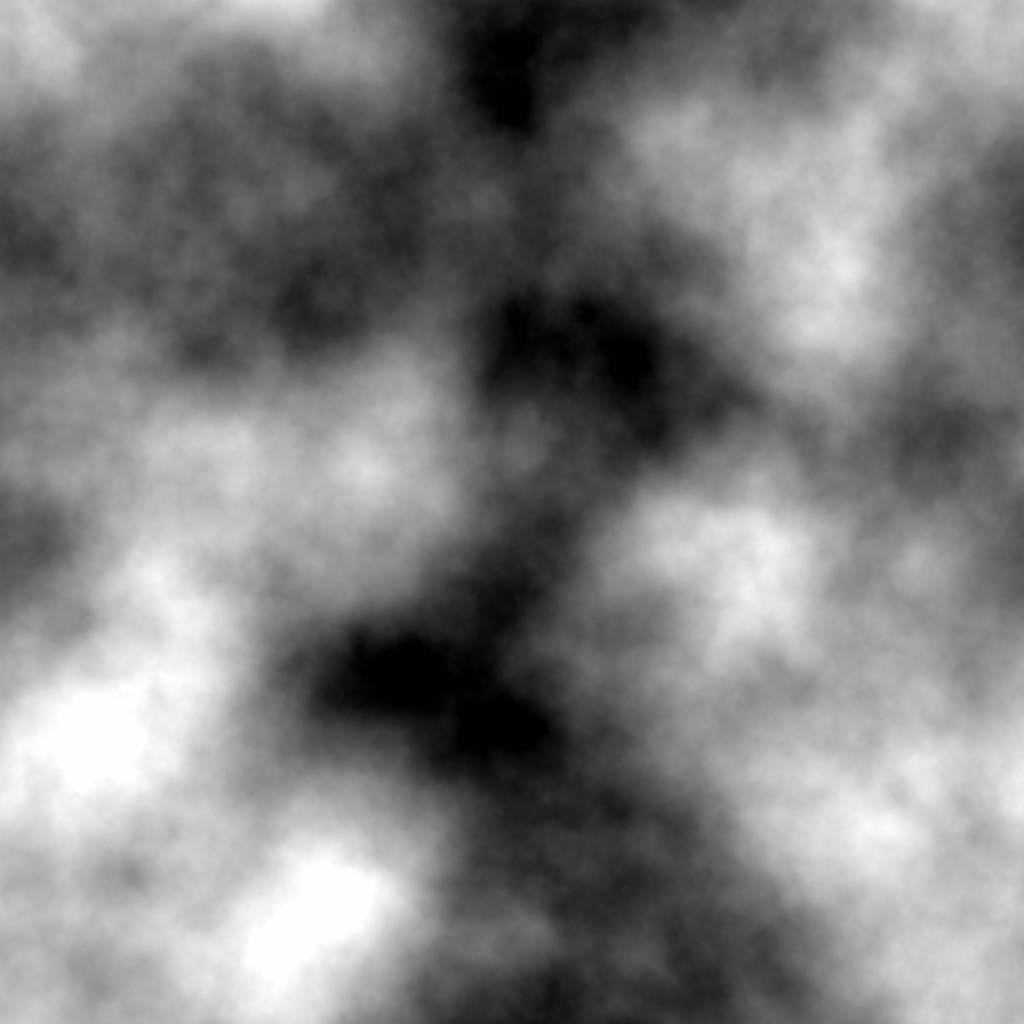
\includegraphics[width=.8\linewidth]{img/brown_noise}
  \caption{Červený, někdy též Brownův šum} 
\end{subfigure}%
\end{tabular} 
\caption{Ukázky různých šumů.} 
\label{obr:noise:example} 
 
\end{figure}
\section{Gabor patch}

Gabor filter (v českých textech někdy označovaný jako Gaborova vlnka) je
lineární filtr používaný ve zpracování obrazu, chceme-li detekovat signál
mající danou frekvenci a směr, který se vyskytuje kolem daného bodu.

\subsection{Definice}

Hodnotu filtru v daném bodě spočítáme jako součin dvou funkcí. První z nich je
vždy sinus či cosinus (někdy uváděné v podobě komplexní exponenciály, pokud
potřebujeme i reálnou, i imaginární složku). Jeho parametry určují, jaké
vlastnosti má mít signál, který chceme detekovat. Druhé funkci říkáme obálka, a
určuje, na jakém okolí daného bodu signál zkoumáme.

Funkce tedy vypadá jako $$g(x,y) =
\sin\left(2\pi\frac{x'}{\lambda}+\phi\right)*\operatorname{obálka}(x',y'),$$
kde vektor $(x',y')^T$ je vektor $(x,y)^T$ otočený o úhel, který svírá osa $x$
se směrem, podél nějž chceme měřit signál (tento úhel budeme značit $\Theta$),
a posunutý do bodu, v němž chceme měřit signál, $\lambda$ je frekvence signálu,
který hledáme, a $\phi$ je fázový posun.

Jako obálka se používá dvojrozměrná Gaussova funkce, raised cosine, nebo prostá lineární funkce vzdálenosti. 

Gaussovu funkci vyjádříme jako $$ \operatorname{obálka}(x,y) =  \exp\left(\frac{x'^2 +
y'^2}{2\rho}\right),$$ kde $\rho$ je směrodatná odchylka Gaussovy křivky. Její výhodou je, že chování Gabor filtru, jehož obálku tvoří Gaussova funkce, je nejlépe popsané. Raised cosine vyjádříme jako 
$$
\operatorname{obálka}(x,y)=
\begin{cases}
 \frac{\cos(\pi\sqrt{x'^2+y'^2}/r)+1}2 &\text{pro $\sqrt{x'^2+y'^2}\leq r$,}\\[1ex]
 0 &\text{jinak,}
\end{cases}
$$ kde $r$ je poloměr oblasti, v níž chceme signál detekovat. Výhodou raised cosine oproti Gaussově funkci je, že ve vzdálenosti alespoň $r$ od středu filtru jeho hodnota nabývá nuly. Při výpočtech tedy stačí počítat s malou oblastí kolem středu (kdežto při použití Gaussovy funkce je nutné počítat s celým obrazem). Výhodou oproti lineární funkci vzdálenosti je, že raised cosine se pro většinu aplikací chová dostatečně podobně, jako Gaussova funkce.

\subsection{Použití}

Chceme-li detekovat signál ve vizuálním šumu, spočítáme hodnotu $$s=\sum g(x,y)*n[x,y],$$ kde $n$ je šum a sumu bereme přes všechny body $(x,y)$, v nichž jsme naměřili hodnoty šumu. Je-li hodnota $s$  blízko nuly, signál v daném místě
není přítomen, nebo je přítomen s jinými parametry. Vysoké hodnoty značí, že
signál pravděpodobně přítomen je, hluboce záporné značí, že signál je přítomen,
ovšem s fází posunutou $\pi$.

Gabor filter ale můžeme používat i k samotné tvorbě signálu. Chceme-li vytvořit
v nějakém bodě signál, můžeme spočítat Gabor filter, jako bychom chtěli
detekovat signál s právě takovými parametry, jaké má mít tvořený signál, a potom ho sečíst se šumem. Takto vytvořenému signálu budeme říkat
Gabor patch.

\begin{figure}[h!]
\begin{subfigure}{0.25\textwidth}
  \centering
  
\includegraphics[width=.8\linewidth]{img/gabor1}
\end{subfigure}% 
\begin{subfigure}{0.25\textwidth}
  \centering
  
\includegraphics[width=.8\linewidth]{img/gabor2}
\end{subfigure}% 
\begin{subfigure}{0.25\textwidth}
  \centering
  
\includegraphics[width=.8\linewidth]{img/gabor3}
\end{subfigure}% 
\begin{subfigure}{0.25\textwidth}
  \centering
  
\includegraphics[width=.8\linewidth]{img/gabor4}
\end{subfigure}% 
\caption{Ukázky několika Gabor patchů. Všechny gabor patche jsou 100 pixelů široké i vysoké. Levý patch má $\Theta = 1/4\pi$, ostatní mají $\Theta = -1/4\pi$, levý má jako obálku Gaussovu funkci, prostřední dva raised cosine, pravý lineární funkci vzdálenosti, první, druhý a čtvrtý mají frekvenci (v cyklech na pixel) $0.1$, třetí $0.02$.} 
\label{obr:gabor:example} 
 
\end{figure}


\section{Ideální bayesovský pozorovatel}

\chapter{Metody}

\TODO{Nemělo by být napřed formálně popsáno, co to vlastně zkoumáme, než začneme popisovat metody?}

\section{Účastníci}

\section{Nástroje a stimuly}

\begin{figure}
\centering
\begin{tabular}{c}
\begin{subfigure}{0.8\textwidth}
\centering
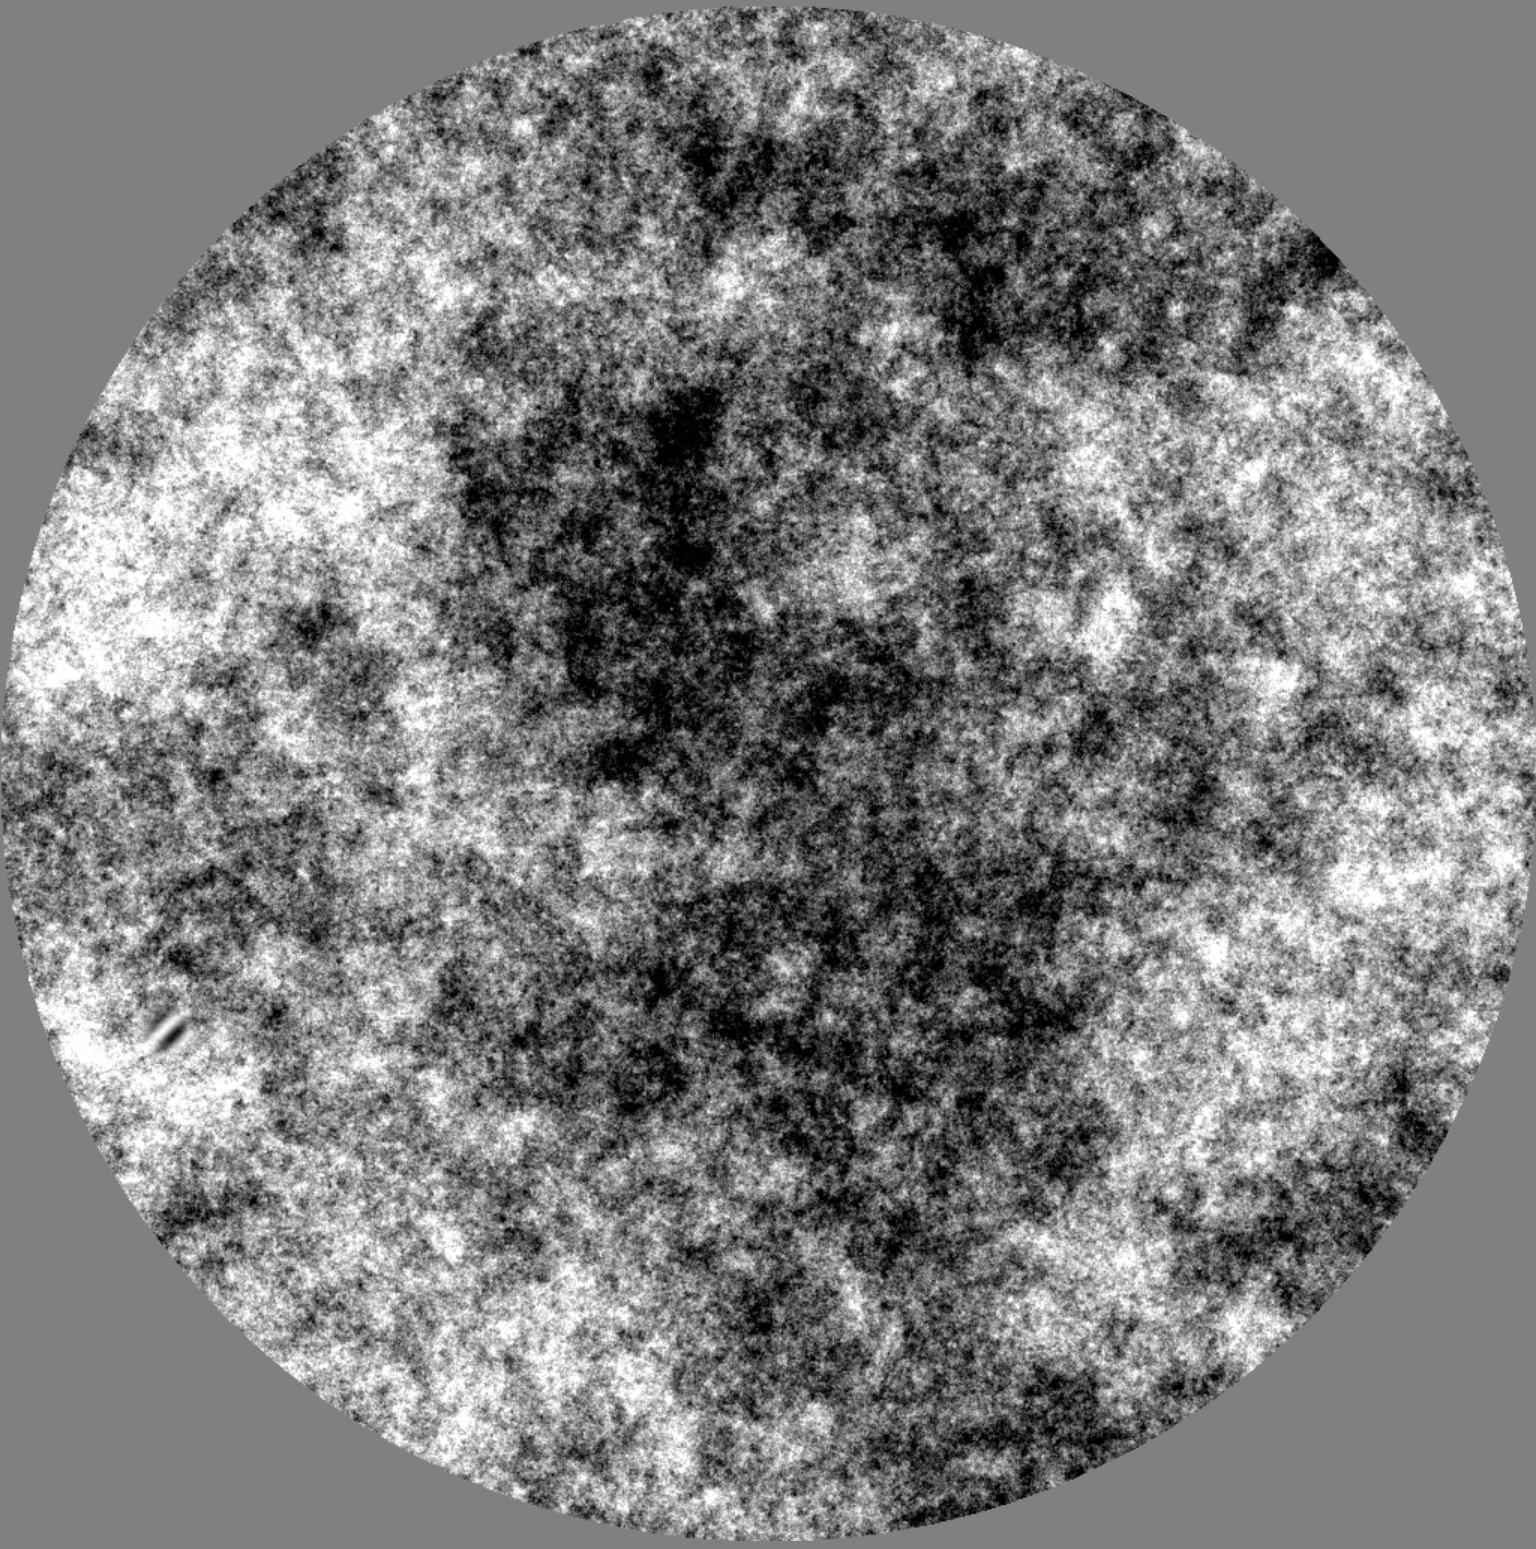
\includegraphics[width = .9\linewidth]{img/noise_visible}
\caption{Šum s dobře viditelným Gabor patchem u levého dolního okraje (kontrast $0.99$).}
\end{subfigure}\\
\begin{subfigure}{0.8\textwidth}
\centering
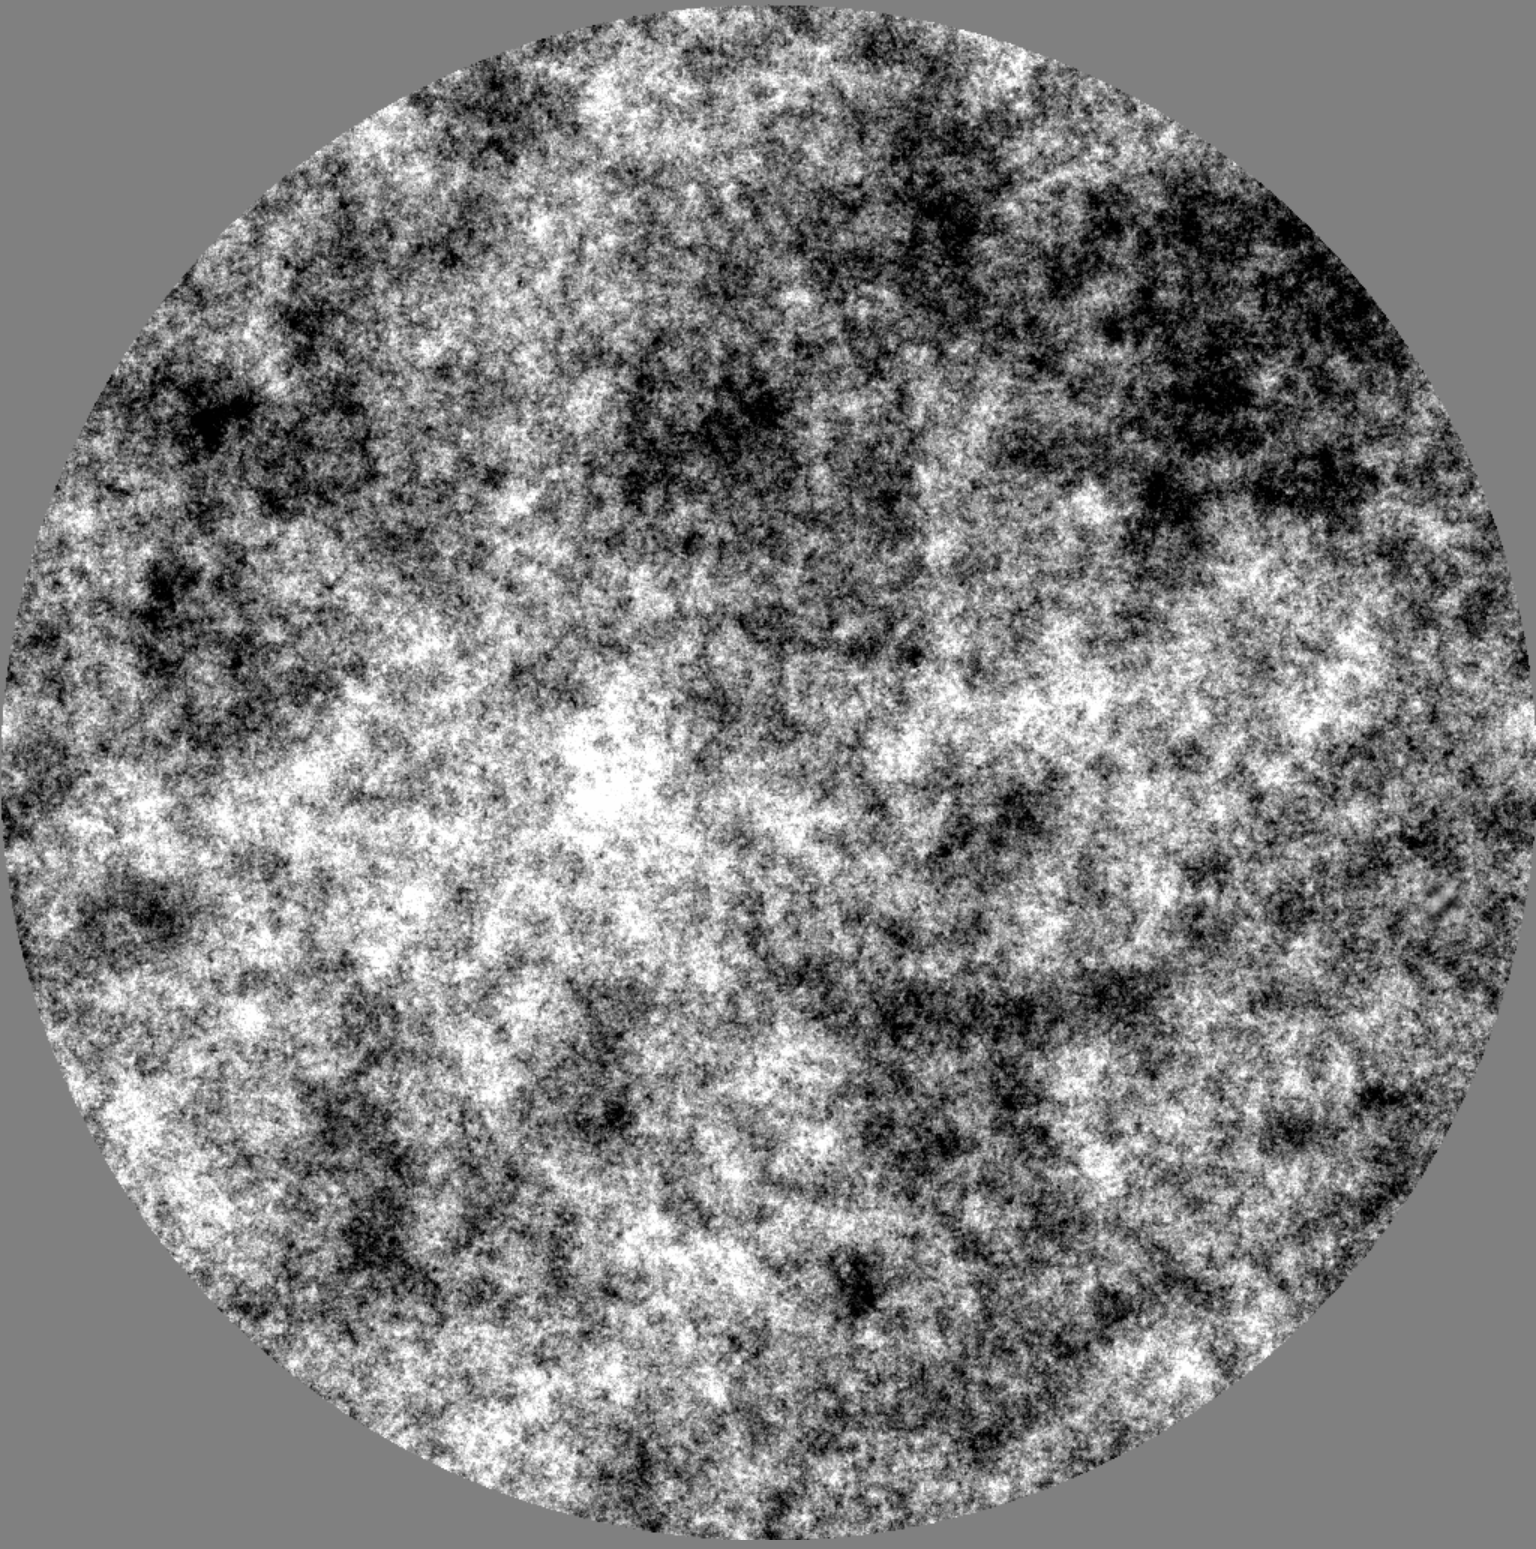
\includegraphics[width = .9\linewidth]{img/noise_invisible}
\caption{Šum se špatně viditelným Gabor patchem u pravého okraje (kontrast $0.61$).}
\end{subfigure}
\end{tabular}
\caption{Příklady šumů s cíli.}
\end{figure}

K experimentu byla použita aplikace, která je součástí této práce. 
Jako zobrazovací zařízení byl použit iPad air s displejem o rozlišení
$2048\times1536$ a o úhlopříčce $9.7$ palců, což odpovídá rozměrům displeje asi
$19.7 \times 14.8$ centimetrů. Hustota pixelů je 264 pixelů na palec. 

V experimentu použitý růžový šum byl kruhový a jeho průměr byl 1024 pixelů.
\footnote{Odsud již všude, kde není zřejmý opak, se pixelem myslí
pixel obrázku, nikoliv pixel displeje.} Tento průměr byl zvolen proto, že je
to nejbližší mocnina dvojky ke kratšímu rozměr displeje iPadu v pixelech.
Mocnina dvojky byla zvolena kvůli použití rychlé Fourierova transformace při
generování růžového šumu.

Jako stimulus byl použit Gabor patch. Jedním z problémů aditivního Gabor patche
ale je fakt, že jas pixelu je v praxi omezený. Kdybychom tedy přičítali Gabor
patch k šumu v místě, které má samo o sobě vysoký jas, museli bychom jeho nejvyšší
bod snížit tak, aby součet se šumem nepřesáhl maximální hodnotu jasu pixelu.
Obdobný problém bychom měli s oblastí s nízkým jasem. Tento problém byl vyřešen
tak, že Gabor k šumu nebyl ale přičten k šumu, ale vložen do něj, jako
kdybychom kreslili Gabor patch přes šum a obálka zastupovala alfa kanál. To
znamená, že jas pixelu v bodě $x$ byl spočítán jako $S[x] * (1-o[x]) +
G[x]*o[x]$, kde $S[x]$ je hodnota šumu v bodě $x$, a $G[x]$ a $o[x]$ jsou
hodnoty Gaboru a jeho obálky.  Zvolené parametry Gabor patche byly:

\begin{itemize}
\item Obálka: Raised cosine
\item Průměr: 50 pixelů
\item Frekvence: $1/16$ cyklu na pixel
\item Fázový posun: 0
\item Úhel $\Theta$: $135^\circ$ 
\end{itemize}

\begin{figure}
\centering
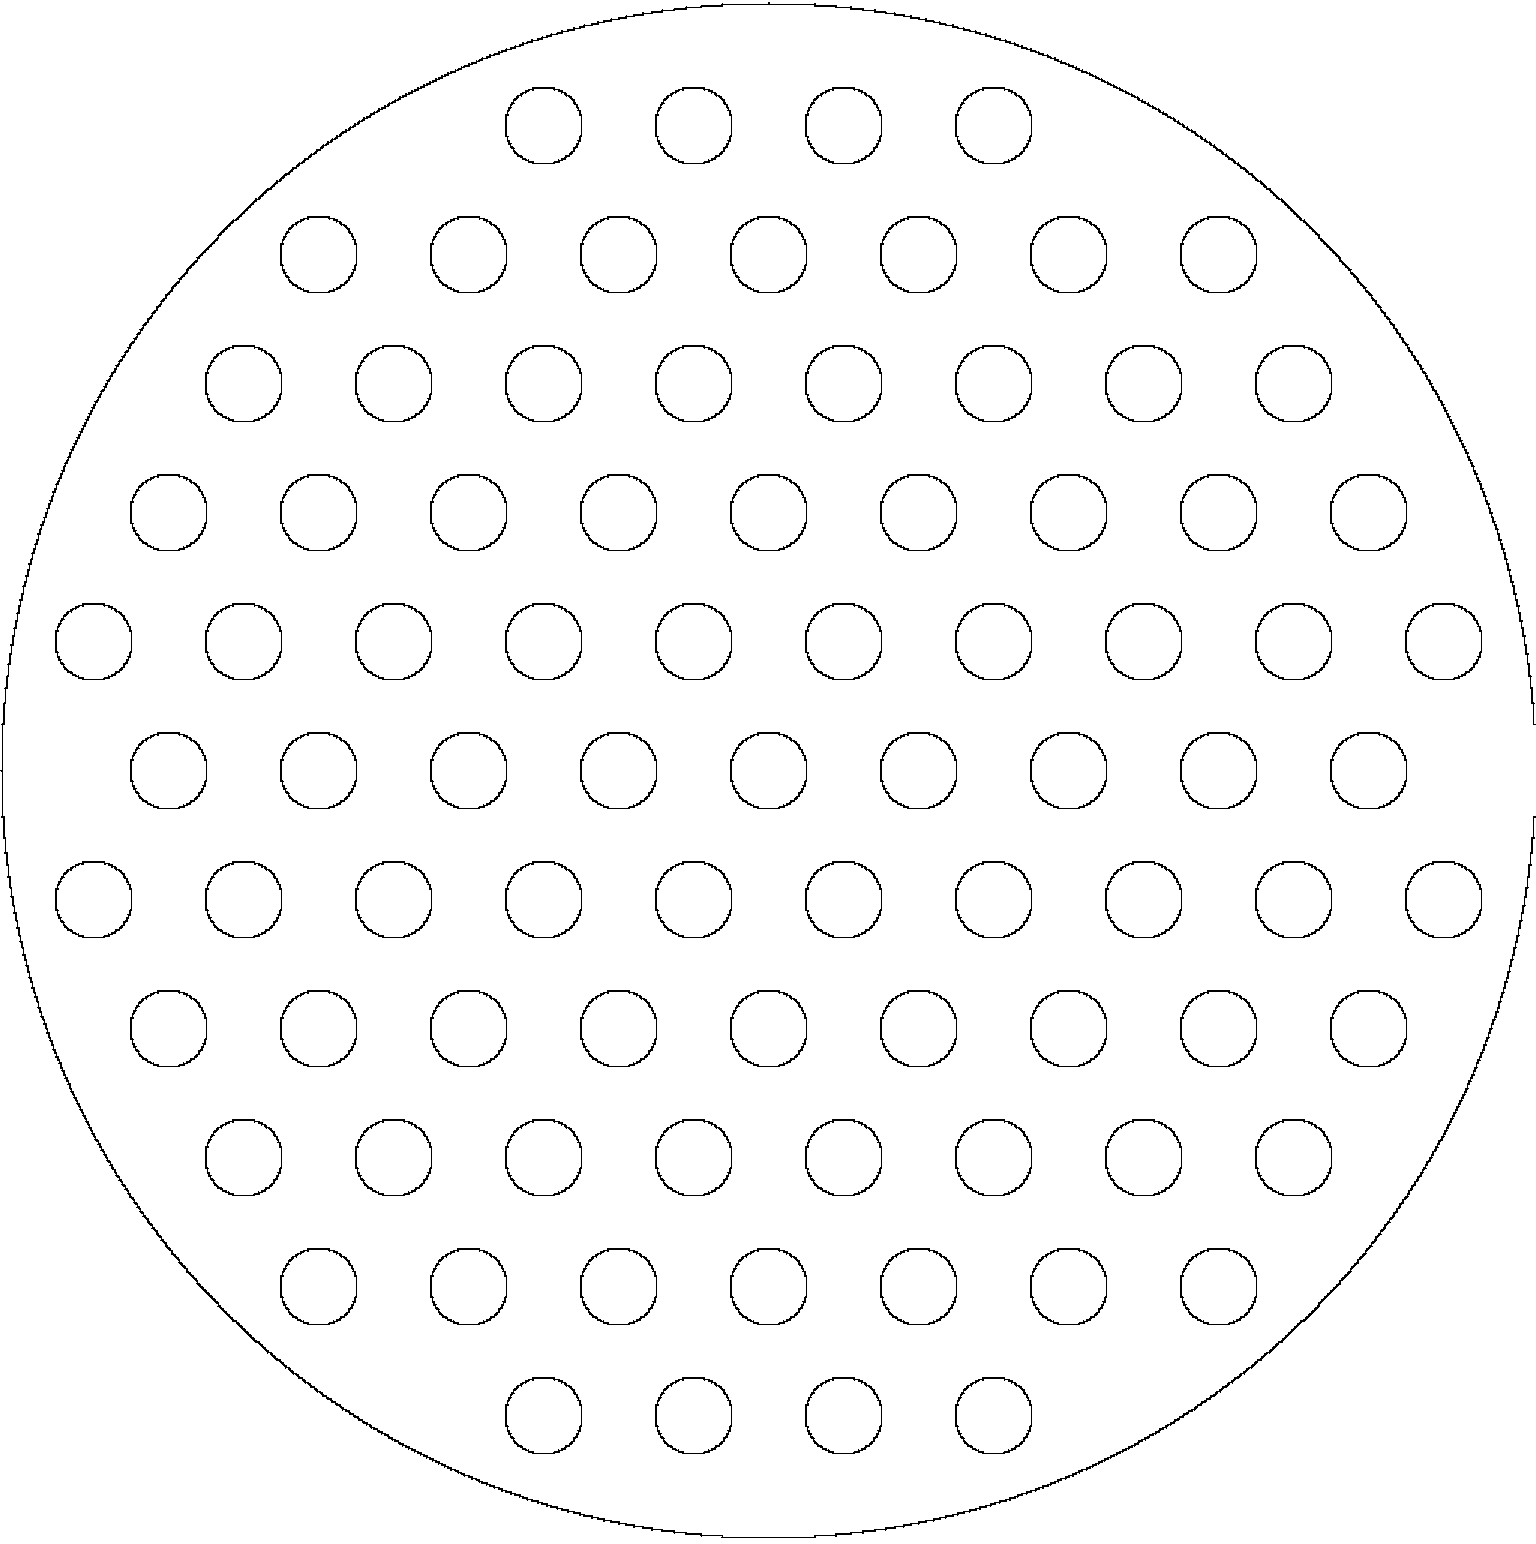
\includegraphics[width=0.48\textwidth]{img/locations_outline.png}
\caption {Možné lokace Gabor patche}.
\end{figure}

Možných lokací Gabor patche bylo celkem 85, a byly rozmístěny po scéně v
trojúhelníkové mřížce tak, aby jedna možná lokace byla ve středu. Vzdálenost
dvou sousedních možných lokací byla 100 pixelů. 

Kontrast cíle byl daný maximem obálky, tedy při snižování kontrastu byl cíl čím dál tím průhlednější. Hodnoty kontrastu se mohly pohybovat mezi nulou a jedničkou.

\section{Procedura}

Každý subjekt prošel sadou 3
testů. V prvním testu mu bylo postupně prezentováno 40 úkolů, kde
v každém z nich měl najít Gabor patch v růžovém šumu.  
V druhém testu bylo prezentováno 120 obdobných úkolů a ve třetím opět 40. Ve druhém testu dostávaly
subjekty, které byly ve skupině se zpětnou vazbou, po každé fixaci zvukovou
odpověď, která značila, kolik informace mohli od této fixace očekávat (tedy
jestli bylo z pohledu ELM moudré udělat právě tuto fixaci). Tato odpověď
byla ve formě tónu, jehož frekvence byla dána vzorcem
$$440\operatorname{Hz}*2^{2-2*\frac{c - \delta}{\Delta - \delta}},$$ kde $c$ je očekávané snížení entropie při fixaci, kterou si subjekt vybral, $\Delta$ je maximální dosažitelné očekávané
snížení entropie a $\delta$ minimální v případě, že by byla zafixována některá
z možných lokací cíle.\footnote{To znamená, že je potenciálně možné dosáhnout
výsledku lepšího než $\Delta$, resp. horšího, než $\delta$. Rozdíl by však
neměl být důležitý.} 

V každém úkolu byl šum překryt černou barvou. Subjekt se měl vždy dotknout displeje v místě, které se
rozhodl zafixovat. Na tomto místě byl poté šum odkryt na $300
\operatorname{ms}$. Výpočet tvaru a míry odkrytí oblasti bylo provedeno
vynásobením s $d'$ mapou posunutou do bodu fixace, s parametrem $d'_0$
nastaveným na 1 a ostatními parametry naměřenými na pozorovateli FD
($e_R=223$, $e_L=223$, $e_U = 161$, $e_D = 164$, $\beta=2.46$, všechny
veličiny, u nichž má smysl uvádět jednotku, jsou v pixelech).

Ve chvíli, kdy si subjekt myslel, že objevil cíl, zmáčkl tlačítko. Poté mu byl ukázán celý odkrytý šum, ovšem
bez cíle. Potom se měl subjekt dotknout šumu na místě, kde si myslel, že se cíl
nacházel. Cíl byl považován za nalezený, pokud byla vzdálenost vybraného místa
a středu skutečné lokace cíle menší než 60 pixelů. Úkol byl považován za úspěšně splněný, pokud byl cíl nalezen a současně v rámci něj účastník provedl nejvýše šest fixací. 

V každém testu byl počáteční kontrast cíle $0.7$. Pokaždé, když byl subjekt třikrát po sobě úspěšný,
byla zvýšena obtížnost snížením kontrastu cíle o $0.01$, pokud byl
třikrát po sobě neúspěšný, byla obtížnost opět snížena. 

Byl tedy využit obecný postup, kterému se říká Up/Down metoda. Tento postup se používá,
pokud je závislost pravděpodobnosti daného jevu na nějakém parametru rostoucí
(či obecně monotónní) funkce. Spočívá v tom, že se daný parametr snižuje, když
jev nastává, a zvyšuje když nenastává (v obou případech o předem danou
konstantu, která se během experimentu nemění, nemusí však být v obou směrech
stejná). Blíže je popsána v knize Psychophysics: A practical introduction \citep{psychophysics}.
Na rozdíl od implementace této metody, která je popsaná v knize, jsme se
rozhodli za jev považovat tři úspěchy za sebou a za jeho absenci tři neúspěchy,
abychom zmenšili velký rozptyl, který náš jev jinak má.\TODO{Nebo jak tohle okecat?}

Hodnota $0.01$ byla vybrána tak, aby se během 120 úkolů, které jsou v prostředním testu, účastník mohl teoreticky dostat až na hodnoty kontrastu kolem $0.3$. S kontrastem menším než přibližně $0.45$ je ale pravděpodobnost splnění úkolu bez ohledu na strategii podle subjektivního názoru autora práce velmi nízká.



\section{Limitace}

Při návrhu experimentu jsme narazili na několik problémů, které mohou vnést
nepřesnosti do měření, ale jejichž řešení je mimo rozsah této práce. Konkrétně
se jedná o následující obtíže:

\begin{itemize}
\item Vjemy lidského pozorovatele neodpovídají příliš dobře vjemům simulovaného
ideálního pozorovatele. Aby si tyto vjemy odpovídaly, alespoň přibližné, museli
bychom každému pozorovateli změřit jeho vlastní $d'$ mapu. Měření $d'$ mapy ale
i  v té nejminimalističtější variantě, která se používá, trvá nejméně jeden
pracovní den. Druhým důvodem, proč mohou být vjemy rozdílné i v případě, že by
konstanty $d'$ mapy vyšly pozorovateli stejně, jaké byly použity, je, že tato
naměřená $d'$ mapa odpovídá situaci, kdy je scéna se šumem umístěna tak daleko
od pozorovatele, aby ji viděl pod zorným úhlem $15^\circ$. To při velikosti
scény v našem případě odpovídá vzdálenosti pozorovatele a zařízení přibližně
$65 \operatorname{cm}$. V našich experimentech nebyla vzdálenost pozorovatele od
scény hlídána. a určitě byla nižší, než řečených $65 \operatorname{cm}$
(dodržení této vzdálenosti by odpovídalo situaci, kdy by subjekty držely iPad
před sebou zhruba na délku natažené paže). 

\item I pokud odhlédneme od nepřesností zmíněných v předchozím bodě a dovolíme
si na chvíli (evidentně scestný) předpoklad, že subjekty měly vlastní $d'$ mapu
konstantní, narazíme na další problém. Okraj oblasti, která byla odkrývána,
byl ztmavován lineárně se snižující se hodnotou $d'$ v použité $d'$ mapě.
Závislost $d'$ na kontrastu ale téměř jistě
není lineární.

\item S tím souvisí ještě jeden problém: Subjekty samozřejmě nemají svou $d'$
mapu konstantní. Tato mapa se tedy nějak skládá s $d'$ mapou, pomocí které
bylo určeno odhalování šumu. V práci jsme toto skládání ignorovali (tedy
předpokládali jsme, že $d'$ na kontrastu závisí lineárně a $d'$ mapa subjektů
je konstantní.) Nabízela by se otázka, proč tedy bylo zatemňování šumu vůbec
prováděno. To se dělo z několika důvodů:

\begin{itemize}

\item Zatemňování šumu zavádí potřebu klikat na místa, která chce pozorovat v
dalším kroku prozkoumat. Nutí tedy pozorovatele, aby tato rozhodnutí dělal
vědomě a nikoli podvědomě, což byl jeden z efektů, které jsme chtěli zkoumat.

\item Celý proces jedné fixace tímto způsobem také trvá mnohem déle (nižší
jednotky vteřin místo nižších desetin vteřiny) a poskytuje nám tedy mnoho času
na update mapy aposteriorních pravděpodobností a výpočet množství informace,
kterou lze získat následující fixací.

\item Takto navržený experiment též umožňuje zjišťovat, které lokace subjekt
fixuje bez použití eyetrackeru nebo jiných technologií.

\end{itemize}

\item Je možné, že u lidí, kteří nikdy dříve Gabor patch hledat nezkoušeli, se
během testů mění jejich senzitivita na Gabor patch (mění se hodnota $d'(0,0)$).

\item Vzhledem k tomu, že počet reálných pixelů displeje neodpovídal (a ani
nebyl dělitelný) velikostí scény v pixelech, je možné, že byly efekty jako
například antialiasing změněny lokální kontrasty scény.

\item Ve výzkumu v oblasti psychofyziky se většinou
pečlivě kontroluje prostředí (například se zatemňuje místnost, v níž se provádí experiment). To jsme v našem výzkumu nedělali.

\end{itemize}

Tyto nepřesnosti však nepovažujeme za příliš důležité, protože cílem této práce
není přesný experiment, ale pouze proof of concept. Za zásadní chybu naopak
nepovažujeme malý počet účastníků -- kdybychom chtěli na této práci postavit
přesný experiment, nebylo by potřeba zvyšovat počet účastníků, ale pouze počet
měření na jednotlivých účastnících, například tak, že bychom vícekrát opakovali
první a třetí test. Jinak ale není ve výzkumu nutně přínosné velký vzorek,
často je lepší na malém vzorku provést větší počet přesnějších měření
\citep{SmallN}. Kdybychom se však rozhodli raději pro Large-$N$ design, mohli
bychom většinu ostatních parametrů experimentu ponechat, ale bylo by potřeba
přinejmenším o řád více účastníků. 


\chapter{Měření}

V této kapitole stručně představíme výsledky měření, detailní grafy ke každému pozorovateli zvlášť jsou v první příloze této práce.

\section{Výsledky}
\begin{figure}[h!]
\centering
\begin{tabular}{c}
\begin{subfigure}{0.80\textwidth}
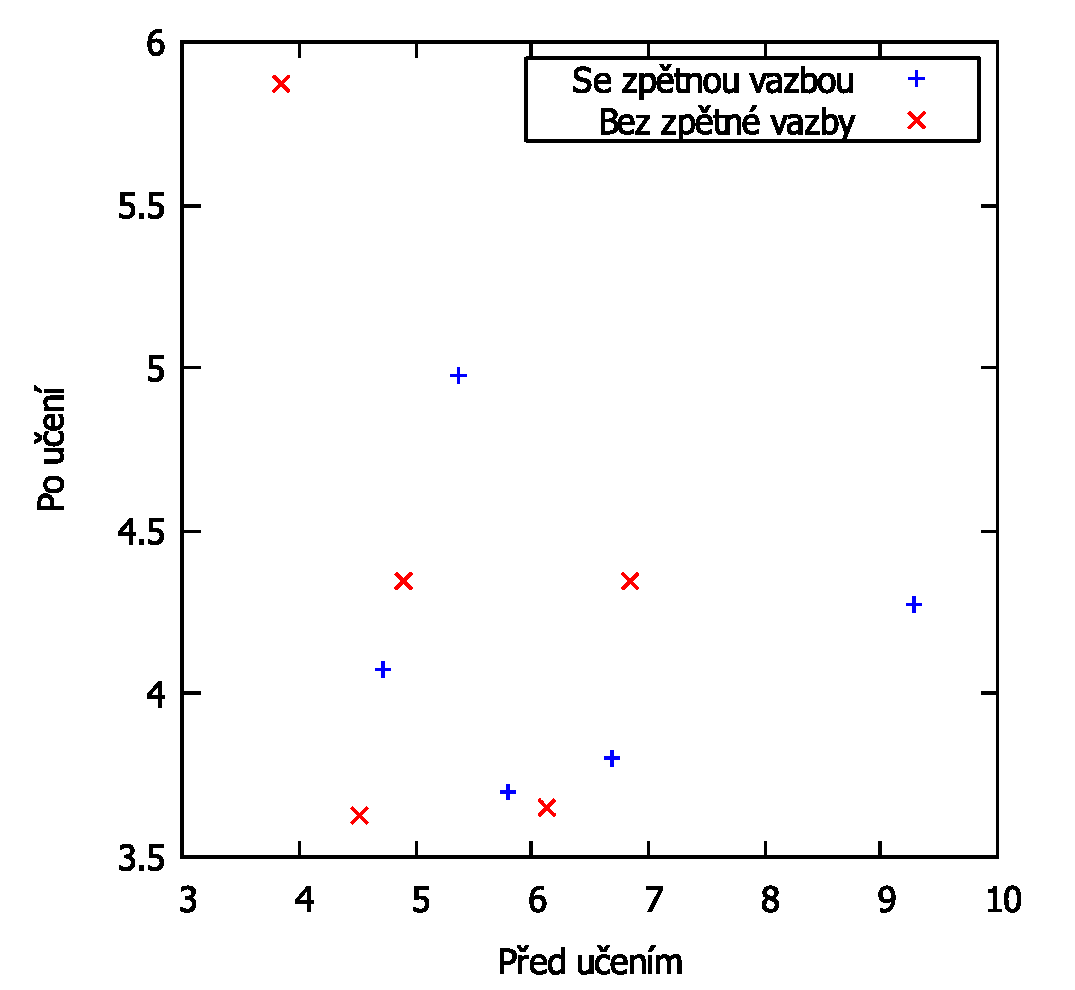
\includegraphics[width=0.99\linewidth]{graphs/AverageTries}
\caption{Průměrný počet fixací}
\end{subfigure}\\
\end{tabular}
\end{figure}
\begin{figure}[h!]
\begin{tabular}{c}
\begin{subfigure}{0.80\textwidth}
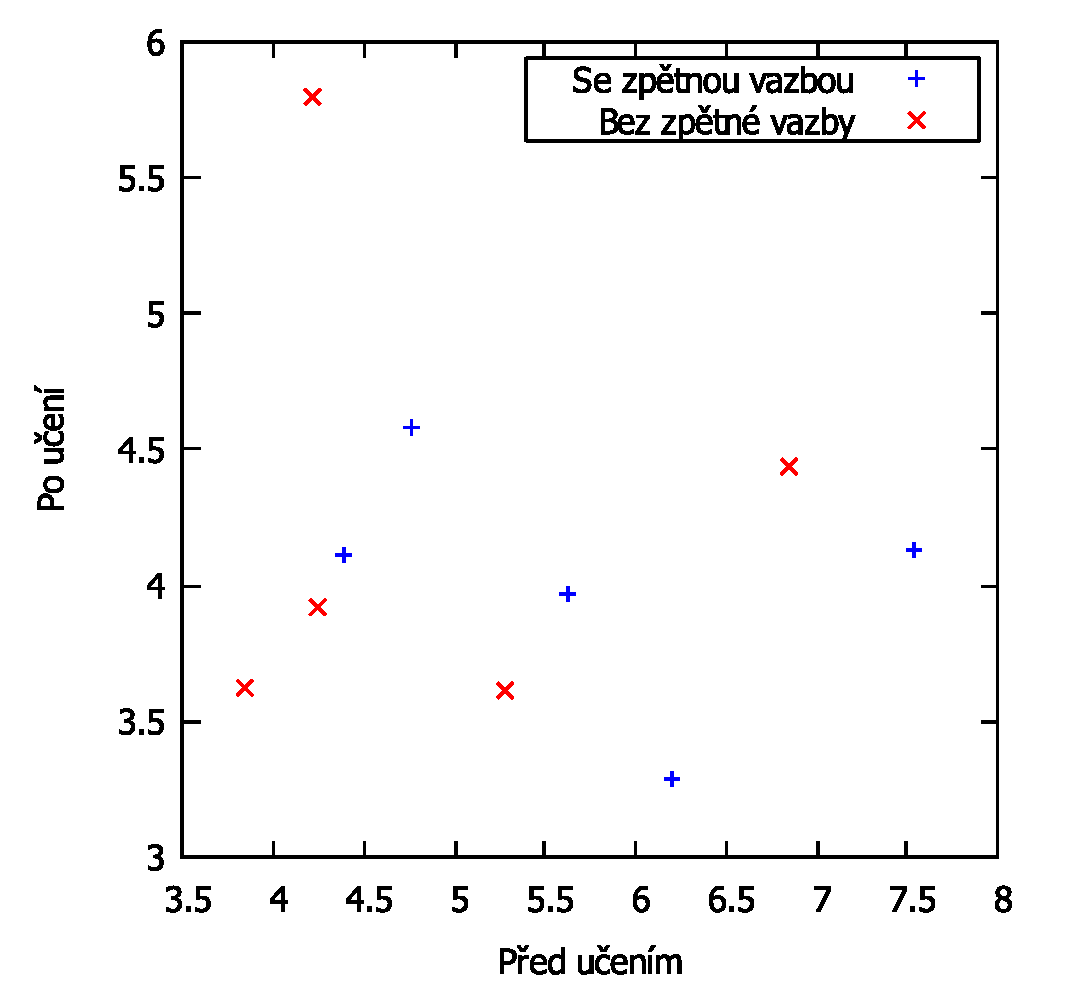
\includegraphics[width=0.99\linewidth]{graphs/AverageSuccesfullTries}
\caption{Průměrný počet fixací v úspěšně splněných úkolech}
\end{subfigure}\\

\begin{subfigure}{0.80\textwidth}
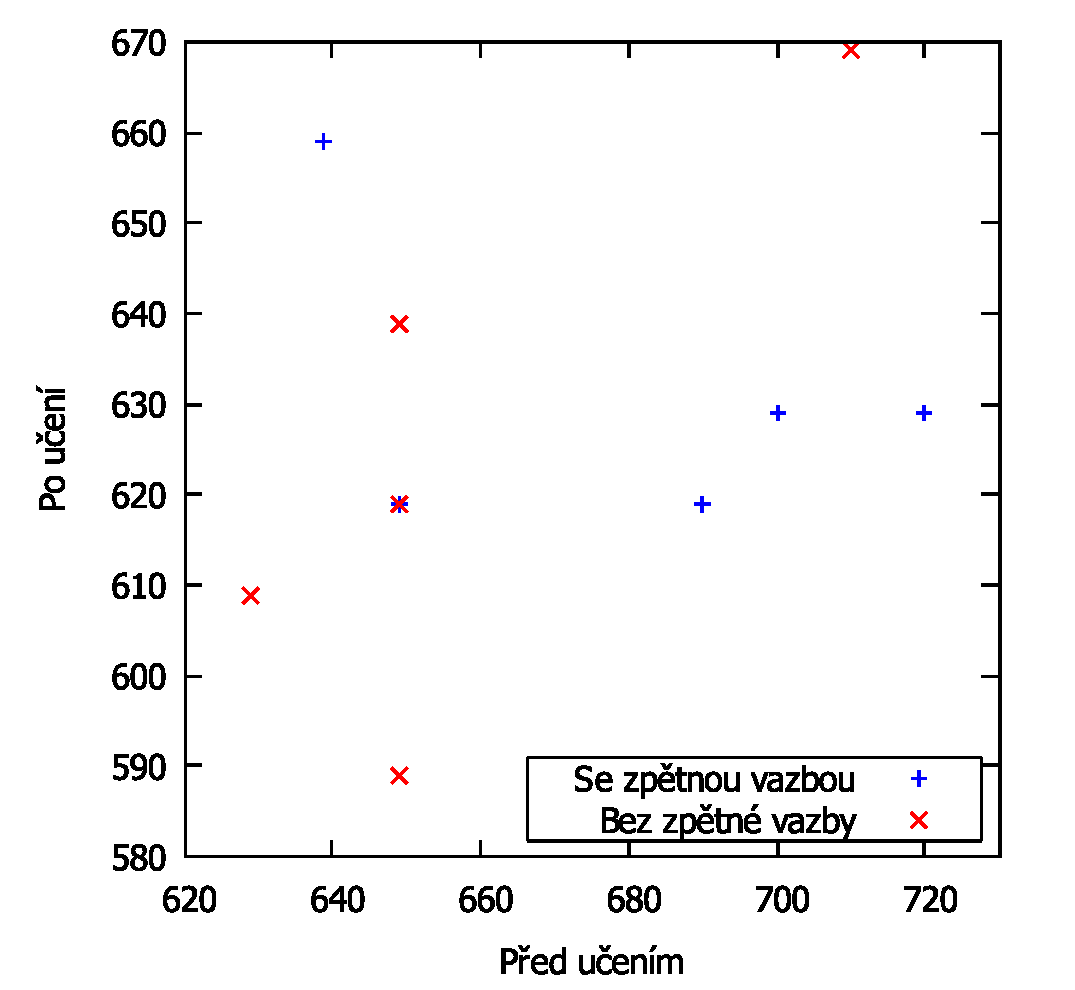
\includegraphics[width=0.99\linewidth]{graphs/FinalDifficulty}
\caption{Obtížnost po 40. pokusu}
\end{subfigure}\\


\end{tabular}
\end{figure}

%%% Fiktivní kapitola s instrukcemi k PDF/A

\chapter{Formát PDF/A}

Opatření rektora č. 13/2017 určuje, že elektronická podoba závěrečných
prací musí být odevzdávána ve formátu PDF/A úrovně 1a nebo 2u. To jsou
profily formátu PDF určující, jaké vlastnosti PDF je povoleno používat,
aby byly dokumenty vhodné k~dlouhodobé archivaci a dalšímu automatickému
zpracování. Dále se budeme zabývat úrovní 2u, kterou sázíme \TeX{}em.

Mezi nejdůležitější požadavky PDF/A-2u patří:

\begin{itemize}

\item Všechny fonty musí být zabudovány uvnitř dokumentu. Nejsou přípustné
odkazy na externí fonty (ani na \uv{systémové}, jako je Helvetica nebo Times).

\item Fonty musí obsahovat tabulku ToUnicode, která definuje převod z~kódování
znaků použitého uvnitř fontu to Unicode. Díky tomu je možné z~dokumentu
spolehlivě extrahovat text.

\item Dokument musí obsahovat metadata ve formátu XMP a je-li barevný,
pak také formální specifikaci barevného prostoru.

\end{itemize}

Tato šablona používá balíček {\tt pdfx,} který umí \LaTeX{} nastavit tak,
aby požadavky PDF/A splňoval. Metadata v~XMP se generují automaticky podle
informací v~souboru {\tt prace.xmpdata} (na vygenerovaný soubor se můžete
podívat v~{\tt pdfa.xmpi}).

Validitu PDF/A můžete zkontrolovat pomocí nástroje VeraPDF, který je
k~dispozici na \url{http://verapdf.org/}.

Pokud soubor nebude validní, mezi obvyklé příčiny patří používání méně
obvyklých fontů (které se vkládají pouze v~bitmapové podobě a/nebo bez
unicodových tabulek) a vkládání obrázků v~PDF, které samy o~sobě standard
PDF/A nesplňují.

Další postřehy o~práci s~PDF/A najdete na \url{http://mj.ucw.cz/vyuka/bc/pdfaq.html}.


\chapter*{Závěr}
\addcontentsline{toc}{chapter}{Závěr}

V~práci jsme představili úlohu zrakového vyhledávání, modely několika pozorovatelů
řešících jednu instanci této úlohy a několik dalších souvisejících konceptů a
teorií. Dále jsme popsali principy percepčního učení.

Poté jsme představili hypotézu, která říkala, že se lidé dokážou naučit řešit
úlohu zrakového vyhledávání lépe, pokud budou dostávat po každém pohledu
zpětnou vazbu. Navrhli jsme experiment, ve kterém jsme se snažili tuto hypotézu
potvrdit či vyvrátit. Ten spočíval v~tom, že jsme nechali účastníky experimentu
opakovaně hledat cíl ve scéně s~vizuálním šumem. Nejprve jsme na několika
takových úkolech změřili výkonnost pozorovatele, potom jsme nechali účastníky
na další sadě úkolů trénovat a nakonec jsme opět změřili jejich výkonnost.
Někteří z~nich přitom dostávali ve fázi tréninku při každé fixaci zvukovou
zpětnou vazbu popisující, jak vhodnou lokaci si uživatel k~fixaci vybral.
K~hodnocení byl použit jeden z~modelů pozorovatelů, konkrétně ELM pozorovatel, který efektivně aproximuje Ideálního Bayesovského pozorovatele.

Vytvořili jsme aplikaci pro operační systém iOS, která gamifikuje úlohu zrakového vyhledávání. Poté jsme s její pomocí provedli navržený experiment. I~přesto, že jsme experiment prováděli pouze na deseti
účastnících (a tedy jsme porovnávali dvě pětičlenné skupiny), podařilo se nám
získat statisticky významný výsledek ($p$-hodnota $0.002$), který říká, že při
opakovaném absolvování úlohy zrakového vyhledávání dochází ke zlepšení výkonu.

Pozitivní vliv zpětné vazby, ač pravděpodobně též velký ($\eta^2_p = 0.17$), se nám však již nejspíše kvůli
malému vzorku a velkému množství vnějšího šumu při experimentech
nepodařilo prokázat. Bylo by zajímavé opakovat experiment s~několika drobnými
změnami, které jsme navrhli při zpracování a diskutování naměřených hodnot.
Výsledky jednotlivých skupin jsou však dostatečně rozdílné na to, abychom věřili, že pokračování
výzkumu tímto směrem má smysl.


%%% Seznam použité literatury
%%% Seznam použité literatury (bibliografie)
%%%
%%% Pro vytváření bibliografie používáme bibTeX. Ten zpracovává
%%% citace v textu (např. makro \cite{...}) a vyhledává k nim literaturu
%%% v souboru literatura.bib.
%%%
%%% Příkaz \bibliographystyle určuje, jakým stylem budou citovány odkazy
%%% v textu. V závorce je název zvoleného souboru .bst. Styly plainnat
%%% a unsrt jsou standardní součástí latexových distribucí. Styl czplainnat
%%% je dodáván s touto šablonou a bibTeX ho hledá v aktuálním adresáři.

\bibliographystyle{czplainnat}    %% Autor (rok) s českými spojkami
% \bibliographystyle{plainnat}    %% Autor (rok) s anglickými spojkami
% \bibliographystyle{unsrt}       %% [číslo]

\renewcommand{\bibname}{Seznam použité literatury}

%%% Vytvoření seznamu literatury. Pozor, pokud jste necitovali ani jednu
%%% položku, seznam se automaticky vynechá.

\bibliography{literatura}

%%% Kdybyste chtěli bibliografii vytvářet ručně (bez bibTeXu), lze to udělat
%%% následovně. V takovém případě se řiďte normou ISO 690 a zvyklostmi v oboru.

% \begin{thebibliography}{99}
%
% \bibitem{lamport94}
%   {\sc Lamport,} Leslie.
%   \emph{\LaTeX: A Document Preparation System}.
%   2. vydání.
%   Massachusetts: Addison Wesley, 1994.
%   ISBN 0-201-52983-1.
%
% \end{thebibliography}


\problemy
%%% Obrázky v bakalářské práci
%%% (pokud jich je malé množství, obvykle není třeba seznam uvádět)
\listoffigures

%%% Tabulky v bakalářské práci (opět nemusí být nutné uvádět)
%%% U matematických prací může být lepší přemístit seznam tabulek na začátek práce.
%\listoftables

%%% Použité zkratky v bakalářské práci (opět nemusí být nutné uvádět)
%%% U matematických prací může být lepší přemístit seznam zkratek na začátek práce.
\printindex
%%% Přílohy k bakalářské práci, existují-li. Každá příloha musí být alespoň jednou
%%% odkazována z vlastního textu práce. Přílohy se číslují.
%%%
%%% Do tištěné verze se spíše hodí přílohy, které lze číst a prohlížet (dodatečné
%%% tabulky a grafy, různé textové doplňky, ukázky výstupů z počítačových programů,
%%% apod.). Do elektronické verze se hodí přílohy, které budou spíše používány
%%% v elektronické podobě než čteny (zdrojové kódy programů, datové soubory,
%%% interaktivní grafy apod.). Elektronické přílohy se nahrávají do SISu a lze
%%% je také do práce vložit na CD/DVD. Povolené formáty souborů specifikuje
%%% opatření rektora č. 72/2017.
\appendix
\chapter*{Přílohy}

\section{První příloha}

\openright
\end{document}
